
\documentclass{article}
\usepackage[landscape]{geometry}
\usepackage{url}
\usepackage{multicol}
\usepackage{amsmath}
\usepackage{esint}
\usepackage{amsfonts}
\usepackage{tikz}
\usetikzlibrary{decorations.pathmorphing}
\usepackage{amsmath,amssymb}

\usepackage{colortbl}
\usepackage{xcolor}
\usepackage{mathtools}
\usepackage{amsmath,amssymb}
\usepackage{enumitem}
\makeatletter

\newcommand*\bigcdot{\mathpalette\bigcdot@{.5}}
\newcommand*\bigcdot@[2]{\mathbin{\vcenter{\hbox{\scalebox{#2}{$\m@th#1\bullet$}}}}}
\makeatother

\title{MATH 2LA3 (Applications of Linear Algebra): Midterm 1 Cheat Sheet}
\usepackage[brazilian]{babel}
\usepackage[utf8]{inputenc}

\advance\topmargin-.8in
\advance\textheight3in
\advance\textwidth3in
\advance\oddsidemargin-1.5in
\advance\evensidemargin-1.5in
\advance\paperheight1.5in % here is new https://tex.stackexchange.com/questions/649149/cheat-sheet-using-mini-pages-and-tikzpicture-does-not-overflow-properly

\makeatletter  % for augmanted matrix from https://tex.stackexchange.com/questions/2233/whats-the-best-way-make-an-augmented-coefficient-matrix
\renewcommand*\env@matrix[1][*\c@MaxMatrixCols c]{%
  \hskip -\arraycolsep
  \let\@ifnextchar\new@ifnextchar
  \array{#1}}
\makeatother

% these two packages needed for dotted vertical line in augmented matrix
\usepackage{amsmath}
\usepackage{arydshln} 

\usepackage{multirow} % for multi column

\parindent0pt
\parskip2pt
\newcommand{\hr}{\centerline{\rule{3.5in}{1pt}}}
%\colorbox[HTML]{e4e4e4}{\makebox[\textwidth-2\fboxsep][l]{texto}
\begin{document}

\begin{center}{\huge{\textbf{MATH 2LA3: Midterm 1 Cheat Sheet}}}\\
\end{center}
\begin{multicols*}{3}

\tikzstyle{mybox} = [draw=black, fill=white, very thick,
    rectangle, rounded corners, inner sep=10pt, inner ysep=10pt]
\tikzstyle{fancytitle} =[fill=black, text=white, font=\bfseries]

%------------ Orthogonal Matrices ---------------
\begin{tikzpicture}
\node [mybox] (box){%
    \begin{minipage}{0.3\textwidth}
    $Q$ is an orthogonal matrix iff:
    \begin{enumerate}
        \item Columns of $Q$ form an orthogonal set (all orthogonal to each other)
        \item Magnitude of each column = 1
    \end{enumerate}
    Properties:
    \begin{enumerate}
        \item $(Q\vec{x})^T(Q\Vec{z}) = \vec{x}^Tz$ (angle preserving)
        \item $||Q\vec{x}||=||\vec{x}||$ (length preserving)
        \item $Q^T = Q^{-1}$
        \item $\det(Q) = \pm 1$
    \end{enumerate}
    \end{minipage}
};
%------------ Orthogonal Matrices Header ---------------------
\node[fancytitle, right=10pt] at (box.north west) {Orthogonal Matrices};
\end{tikzpicture}

%------------ Markov Chains ---------------
\begin{tikzpicture}
\node [mybox] (box){%
    \begin{minipage}{0.3\textwidth}
    Let $A$ be a regular transition matrix: $A = 
    \begin{bmatrix}
        0.1 & 0.6\\
        0.9 & 0.4
    \end{bmatrix}$
    To find the long term probability the system will be at a particular state, find the eigenvector corresponding to $\lambda = 1$ and scale it to a probability vector $\vec{p}$.\\
    
    $[A | 0] \sim
    \begin{bmatrix}[cc:c]
      1 & \frac{-2}{3} & 0\\
      0 & 0 & 0
    \end{bmatrix}$\\
    
    $\Rightarrow \vec{x} = x_2
    \begin{bmatrix}
        \frac{2}{3}\\
        1
    \end{bmatrix}$\\
    $\Rightarrow \vec{p} = \frac{1}{\frac{2}{3} + 1}
    \begin{bmatrix}
        \frac{2}{3}\\
        1
    \end{bmatrix} = 
    \begin{bmatrix}
        0.4\\
        0.6
    \end{bmatrix}$
    $
    \begin{matrix}
        \leftarrow \text{Long term $P$(in state 1)}\\
        \leftarrow \text{Long term $P$(in state 2)}
    \end{matrix}$
    \end{minipage}
};
%------------ Markov Chains Header ---------------------
\node[fancytitle, right=10pt] at (box.north west) {Markov Chains};
\end{tikzpicture}

%------------ Diagonalization Content ---------------
\begin{tikzpicture}
\node [mybox] (box){%
    \begin{minipage}{0.3\textwidth}
    $D = 
    \begin{bmatrix}
        \lambda_1 & 0 & 0 \\
        0 & \ddots & 0 \\
        0 & 0 & \lambda_n
    \end{bmatrix}$\\
    $P = \begin{bmatrix}
        \vec{\text{eigen}_{\lambda_1}} & \hdots & \vec{\text{eigen}_{\lambda_n}}
    \end{bmatrix}$\\
    $A$ and $D$ are similar and $A$ is diagonalizable iff $A = PDP^{-1}$.\\
    $A$ is diagonalizable iff (equivalent statements):
    \begin{itemize}
        \item $A$ has $n$ linearly independent eigenvectors
        \item $\sum_{i} \text{GM}(\lambda_i) = n$. GM($\lambda$) := number of eigenvectors for eigenvalue $\lambda$
    \end{itemize}
    $A$ diagonalizable $\Leftrightarrow A^n = PD^nP^{-1}$\\
    
    
    \end{minipage}
};
%------------ Diagonalization Header ---------------------
\node[fancytitle, right=10pt] at (box.north west) {Diagonalization};
\end{tikzpicture}

%------------ Orthogonal Compliment ---------------
\begin{tikzpicture}
\node [mybox] (box){%
    \begin{minipage}{0.3\textwidth}
    Definition: if $W$ is a subspace of $\mathbb{R}^n$, then $W^{\perp}$ contains all vectors $\in \mathbb{R}^n$ perpendicular to $W$\\
    Properties:
    \begin{enumerate}
        \item $W^{\perp} =$ Null($A^T$)
        \item dim($W$) + dim($W^{\perp}) = n$
        \item $(W^{\perp})^{\perp} = W$
        \item $W \cap W{^\perp} = \{ \vec{0} \}$
        \item $(\mathbb{R}^n)^{\perp} = \{ \vec{0} \}$; $\{ \vec{0} \}^{\perp} = \mathbb{R}^n$
    \end{enumerate}
    Subspaces of $\mathbb{R}^n$:
    \begin{itemize}
        \item Row($A$) = (Nul($A$))$^{\perp}$
        \item Nul($A$) = (Row($A$))$^{\perp}$
        \item dim(Row($A$)) = Rank($A$)
        \item dim(Nul($A$)) = $n$ - Rank($A$)
    \end{itemize}
    Subspaces of $\mathbb{R}^m$:
    \begin{itemize}
        \item Col($A$) = (Nul($A^T$))$^{\perp}$
        \item Nul($A^T$) = (Col($A$))$^{\perp}$
        \item dim(Col($A$)) = Rank($A$)
        \item dim(Nul($A^T$)) = $m$ - Rank($A$)
    \end{itemize}
    \textbf{Example: find a basis for Row($A$)}\\
    $\vec{v} = \begin{bmatrix} 1\\ 2\\ 1\\ 2 \end{bmatrix}$, and $A\vec{v} = \vec{0}$\\
    $A\vec{v} = \vec{0}$, so $\vec{v} \in$ Nul($A$).\\
    Let $W = $Nul($A$), so $W^\perp =$ Row($A$)\\
    $\Rightarrow $ Nul($\Vec{v}^T$) is a basis for Row($A$).\\
    \begin{align*}
        \text{Nul}(\begin{bmatrix} 1&2&1&2 \end{bmatrix}) &= \left\{ \begin{bmatrix} -2\\ 1\\ 0\\ 0 \end{bmatrix}, \begin{bmatrix} -1\\ 0\\ 1\\ 0 \end{bmatrix}, \begin{bmatrix} -2\\ 0\\ 0\\ 1 \end{bmatrix} \right\} \\
        &= \text{basis for Row}(A)
    \end{align*}
        
    \end{minipage}
};
%------------ Orthogonal Compliment Header ---------------------
\node[fancytitle, right=10pt] at (box.north west) {Orthogonal Compliment};
\end{tikzpicture}



%------------ Vector Spaces and Subspaces Content ---------------------
\begin{tikzpicture}
\node [mybox] (box){%
    \begin{minipage}{0.3\textwidth}
        - Nul($A$) := Solutions to $A\Vec{x} = \vec{0}$. From  RREF($[A|0]$)\\
        % Col($A$) := Space spanned by columns of $A$.
        - Basis of Col($A$) cols of $A$ w/ pivots\\
        - Basis of Row($A$) row vectors of RREF($A$)\\
        CR Factorization: $A = CR$
        \begin{itemize}
            \item $C = [\vec{\text{basis of col(A)}_{1}} \hdots \vec{\text{basis of col(A)}_{k}}]$
            \item $R = RREF(A)$
        \end{itemize}
        Descriptions of a subspace in $\mathbb{R}^n$:\\
        - A span of vectors in $\mathbb{R}^n$ is a subspace of $\mathbb{R}^n$\\
        - $\vec{0}$\\
        - $\mathbb{R}^n$ (any space is a subspace of itself)\\
        - The solution set to $A\vec{x} = \Vec{0}$ for any $n \times n$ matrix $A$\\
        - Any line in $\mathbb{R}^n$ \textbf{Which must pass through the origin}\\
        \textbf{Example:}
        \begin{itemize}
            \item $w_1 \begin{bmatrix} u_1 \\ u_2 \end{bmatrix} + w_2 \begin{bmatrix} v_1 \\ v_2 \end{bmatrix}$ is a subspace (all vectors have weights)
            \item $w_1 \begin{bmatrix} u_1 \\ u_2 \end{bmatrix} + \begin{bmatrix} v_1 \\ v_2 \end{bmatrix}$ isn't a subspace
        \end{itemize}
        
    \end{minipage}
};
%------------ Vector Spaces and Subspaces Header ---------------------
\node[fancytitle, right=10pt] at (box.north west) {Vector Spaces and Subspaces};
\end{tikzpicture}

%------------ Matrix Properties Content ---------------
\begin{tikzpicture}
\node [mybox] (box){%
    \begin{minipage}{0.3\textwidth}
    $A_{m \times n} \Rightarrow $ transformation $\vec{x} \rightarrow A\vec{x}$ is from $\mathbb{R}^n \rightarrow \mathbb{R}^m$\\
    Rank$(A)$ + nullity($A$) = $n$
        \hrule
    
    \small{
    	\begin{tabular}{lp{4cm} l}
		\textbf{Determinants} & $\det(AB) = \det(A)\det(B)$ \\
                & $\det(A^{-1}) = \frac{1}{\det(A)}$ \\
                & $\det(\text{adj}(A)) = \det(A)^{n-1}$ \\
                & $\det(A^n) = ({\det(A)})^n$ \\
                & $\det(cA) = c^n\det(A)$ \\ 
                & $\det(A^T) = \det(A)$ \\ 
                & $\det \begin{bmatrix} a & b \\ c & d \end{bmatrix} = ad - bc$\\
            \hline

		\textbf{Inverse} & $(AB)^{-1} = B^{-1}A^{-1}$ \\
                & $(A^{-1})^{-1} = A$ \\
                & $(kA^{-1}) = \frac{1}{k}A$ \\
                & $(A^{-1})^{-1} = I_n$ \\ 
                
                & \multirow{2}{*}{$\begin{bmatrix} a & b \\ c & d \end{bmatrix}^{-1} = \frac{1}{ad - bc} \begin{bmatrix} d & -b \\ -c & a \end{bmatrix}$} \\
                & \\
                & \\
            \hline
            
		\textbf{Transpose} & $(A^T)^T = A$ \\
                & $(AB)^{T} = B^{T}A^{T}$ \\
                & $(kA^{T}) = kA^T$ \\
                & $(A + B)^T = A^T + B^T$ \\ 
            % \hline
	\end{tabular}}
    \end{minipage}
};
%------------ Matrix Properties Header ---------------------
\node[fancytitle, right=10pt] at (box.north west) {Matrix Properties};
\end{tikzpicture}

%------------ Eigenvalues and Eigenvectors Content ---------------
\begin{tikzpicture}
\node [mybox] (box){%
    \begin{minipage}{0.3\textwidth}
    The Eigenvalues of a triangular or diagonal matrix are along the main diagonal.\\
    To \textbf{Find Eigenvalues} of $A = 
    \begin{bmatrix}
        -5 & 2 \\
        -9 & 6
    \end{bmatrix}$\\
    Solve $ |A-\lambda I_n| = \vec{0} \Leftrightarrow
        \begin{bmatrix}
            -5 - \lambda & 2 \\
            -9 & 6 - \lambda
        \end{bmatrix} = \vec{0}$

    To \textbf{Find Eigenvectors for $\lambda_i$}, solve:\\
        $\begin{bmatrix}[cc:c]
            -5 - \lambda_i & 2 & 0 \\
            -9 & 6 - \lambda_i & 0
        \end{bmatrix}$\\
    - AM($\lambda = 0$) = nullity($A)$
    \end{minipage}
};
%------------ Eigenvalues and Eigenvectors Header ---------------------
\node[fancytitle, right=10pt] at (box.north west) {Eigenvalues and Eigenvectors};
\end{tikzpicture}


%------------ Dot Product Content ---------------
\begin{tikzpicture}
\node [mybox] (box){%
    \begin{minipage}{0.3\textwidth}
    -  $\begin{bmatrix}
        u_1 \\
        u_2
    \end{bmatrix} \cdot
    \begin{bmatrix}
        v_1\\
        v_2
    \end{bmatrix} = (u_1)(v_1) + (u_2)(v_2)
    $\\
    - $\vec{u} \cdot \vec{v} = \vec{u}^T \vec{v}$\\
    - $\vec{u} \cdot \Vec{u} = \left( ||\vec{u}|| \right)^2$\\
    - if $\vec{u} \cdot \vec{v} = 0$, then $\vec{u}$ and $\vec{v}$ are orthogonal\\
    - $(\vec{a} + \vec{b}) \cdot (\vec{c} + \Vec{d}) = \vec{a} \cdot \vec{c} + \vec{a} \cdot \vec{d} + \vec{b} \cdot \vec{c} + \vec{b} \cdot \vec{d}$
    \end{minipage}
};
%------------ Dot Product Header ---------------------
\node[fancytitle, right=10pt] at (box.north west) {Dot Product};
\end{tikzpicture}

%------------ Span Content ---------------
\begin{tikzpicture}
\node [mybox] (box){%
    \begin{minipage}{0.3\textwidth}
    \textbf{Def} The span of a set of vectors is the set of linear combinations of the vectors.\\
    Check if $\vec{w} \in $span$\{\vec{u}, \vec{v} \}$:\\
    $\begin{bmatrix}[cc:c]
            u_1 & v_1 & w_1 \\
            u_2 & v_2 & w_2
        \end{bmatrix}$ $\vec{w} \in $span$\{\vec{u}, \vec{v} \}$ iff that system has a solution.

    Check if span$\{\vec{u}, \vec{v}, \vec{w}\} = \mathbb{R}^3:$\\ (equivalent to col[$\Vec{u}, \vec{v}, \vec{w}$] = $\mathbb{R}^3$)\\
    $\begin{bmatrix}
            u_1 & v_1 & w_1 \\
            u_2 & v_2 & w_2 \\
            u_3 & v_3 & w_3
        \end{bmatrix}$ True iff that matrix has a pivot in each row/column
    \end{minipage}
};
%------------ Span Header ---------------------
\node[fancytitle, right=10pt] at (box.north west) {Span};
\end{tikzpicture}

%------------ Vector Spaces ---------------
\begin{tikzpicture}
\node [mybox] (box){%
    \begin{minipage}{0.3\textwidth}
    $v_1, v_2 \in V$\\
    1. $v_1 + v_2 \in V$ \\
	2. $k \in \mathbb{F}, kv_1 \in V $ \\
	3. $ v_1 + v_2 = v_2 + v_1 $ \\
	4. $(v_1 + v_2) + v_3 = v_1 + (v_2 + v_3) $ \\
	5. $\forall v \in V, 0 \in V \mid 0 + v_1 = v_1 + 0 = v_1$ \\
    6. $\forall v \in V, \exists -v \in V \mid v + (-v) = (-v) + v = 0 $ \\
    7. $\forall v \in V, 1 \in \mathbb{F} \mid 1*v = v$ \\
    8. $\forall v \in V, k,l \in \mathbb{F}, (kl)v = k (lv)$ \\
    9. $\forall k \in \mathbb{F}, k(v_1 + v_2) = kv_1 + kv_2$ \\
    10. $\forall v \in V, k,l \in \mathbb{F}, (k+l)v = kv + lv$
    \end{minipage}
};
%------------ Vector Space Header ---------------------
\node[fancytitle, right=10pt] at (box.north west) {Vector Spaces};
\end{tikzpicture}

%------------ Sample Questions Content ---------------
\begin{tikzpicture}
\node [mybox] (box){%
    \begin{minipage}{0.3\textwidth}
    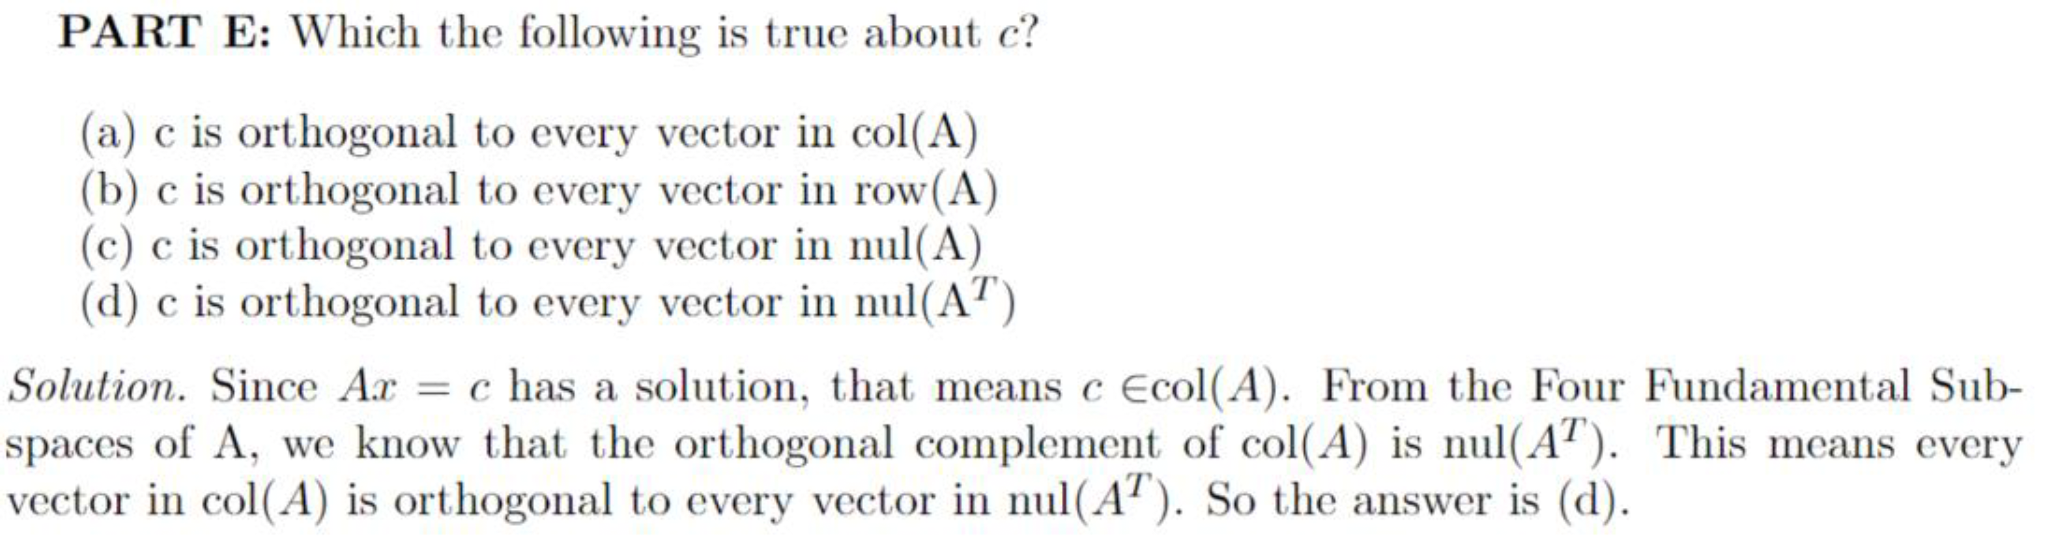
\includegraphics[scale=0.225]{q4_pre_test_lec.png}
    \end{minipage}
};
%------------ Sample Questions Header ---------------------
\node[fancytitle, right=10pt] at (box.north west) {Sample Questions};
\end{tikzpicture}

\end{multicols*}
\end{document}

